\documentclass[main.tex]{subfiles}

\begin{document}
\lhead{Appendix}
\chapter{Result Details}
\section{Fine-tuning hyperparameter search results}
\label{sec:hyperres}

\begin{table}
    \footnotesize
    \begin{tabular}{lllll|rrr}
        Batch size & Learning rate & Weight decay & Dropout & Loss weight & F1    &  Precision & Recall\\\hline
        8& 1\ctp{-5}& 0.01& 0.025& Yes       & 73.06 &  62.82 &  87.29\\
        8& 1\ctp{-5}& 0.01& 0.025& No        & 73.53 &  62.87 &  88.54\\
        8& 1\ctp{-5}& 0.01& 0.1& Yes         & 73.52 &  63.17 &  87.92\\
        8& 1\ctp{-5}& 0.01& 0.1& No          & 71.39 &  60.00 &  88.12\\
        8& 1\ctp{-5}& 0.05& 0.025& Yes       & 72.87 &  62.54 &  87.29\\
        8& 1\ctp{-5}& 0.05& 0.025& No        & 67.77 &  56.07 &  85.62\\
        8& 1\ctp{-5}& 0.05& 0.1& Yes         & 71.44 &  60.46 &  87.29\\
        8& 1\ctp{-5}& 0.05& 0.1& No          & 71.91 &  61.45 &  86.67\\
        8& 5\ctp{-5}& 0.01& 0.025& Yes       & 83.08 &  77.14 &  90.00\\
        8& 5\ctp{-5}& 0.01& 0.025& No        & \textbf{85.35} &  \textbf{80.82} &  90.42\\
        8& 5\ctp{-5}& 0.01& 0.1& Yes         & 84.96 &  80.45 &  90.00\\
        8& 5\ctp{-5}& 0.01& 0.1& No          & 31.53 &  19.86 &  76.46\\
        8& 5\ctp{-5}& 0.05& 0.025& Yes       & 84.00 &  79.41 &  89.17\\
        8& 5\ctp{-5}& 0.05& 0.025& No        & 84.24 &  77.78 &  \textbf{91.88}\\
        8& 5\ctp{-5}& 0.05& 0.1& Yes         & 84.65 &  79.74 &  90.21\\
        8& 5\ctp{-5}& 0.05& 0.1& No          & \textbf{85.35} &  \textbf{80.82} &  90.42\\
        16& 1\ctp{-5}& 0.01& 0.025& Yes      & 65.29 &  52.76 &  85.62\\
        16& 1\ctp{-5}& 0.01& 0.025& No       & 63.91 &  51.12 &  85.21\\
        16& 1\ctp{-5}& 0.01& 0.1& Yes        & 63.33 &  50.24 &  85.62\\
        16& 1\ctp{-5}& 0.01& 0.1& No         & 62.57 &  49.57 &  84.79\\
        16& 1\ctp{-5}& 0.05& 0.025& Yes      & 63.73 &  50.61 &  86.04\\
        16& 1\ctp{-5}& 0.05& 0.025& No       & 63.63 &  50.55 &  85.83\\
        16& 1\ctp{-5}& 0.05& 0.1& Yes        & 64.13 &  51.11 &  86.04\\
        16& 1\ctp{-5}& 0.05& 0.1& No         & 63.06 &  49.70 &  86.25\\
        16& 5\ctp{-5}& 0.01& 0.025& Yes      & 84.83 &  79.10 &  91.46\\
        16& 5\ctp{-5}& 0.01& 0.025& No       & 83.72 &  78.26 &  90.00\\
        16& 5\ctp{-5}& 0.01& 0.1& Yes        & 82.66 &  76.88 &  89.38\\
        16& 5\ctp{-5}& 0.01& 0.1& No         & 29.21 &  18.08 &  76.04\\
        16& 5\ctp{-5}& 0.05& 0.025& Yes      & 83.67 &  77.25 &  91.25\\
        16& 5\ctp{-5}& 0.05& 0.025& No       & 83.60 &  76.70 &  \textbf{91.88}\\
        16& 5\ctp{-5}& 0.05& 0.1& Yes        & 83.29 &  76.90 &  90.83\\
        16& 5\ctp{-5}& 0.05& 0.1& No         & 82.94 &  76.45 &  90.62
    \end{tabular}
    \caption{
        The results of hyperparameter search with micro average percentages for the metrics reported.
    }
    \label{tab:hyperres}
\end{table}
\chapter{Additional Figures}
\section{Dimensionality Reduction}
\label{sec:dimredu}

\begin{figure}[H]
    \centering
        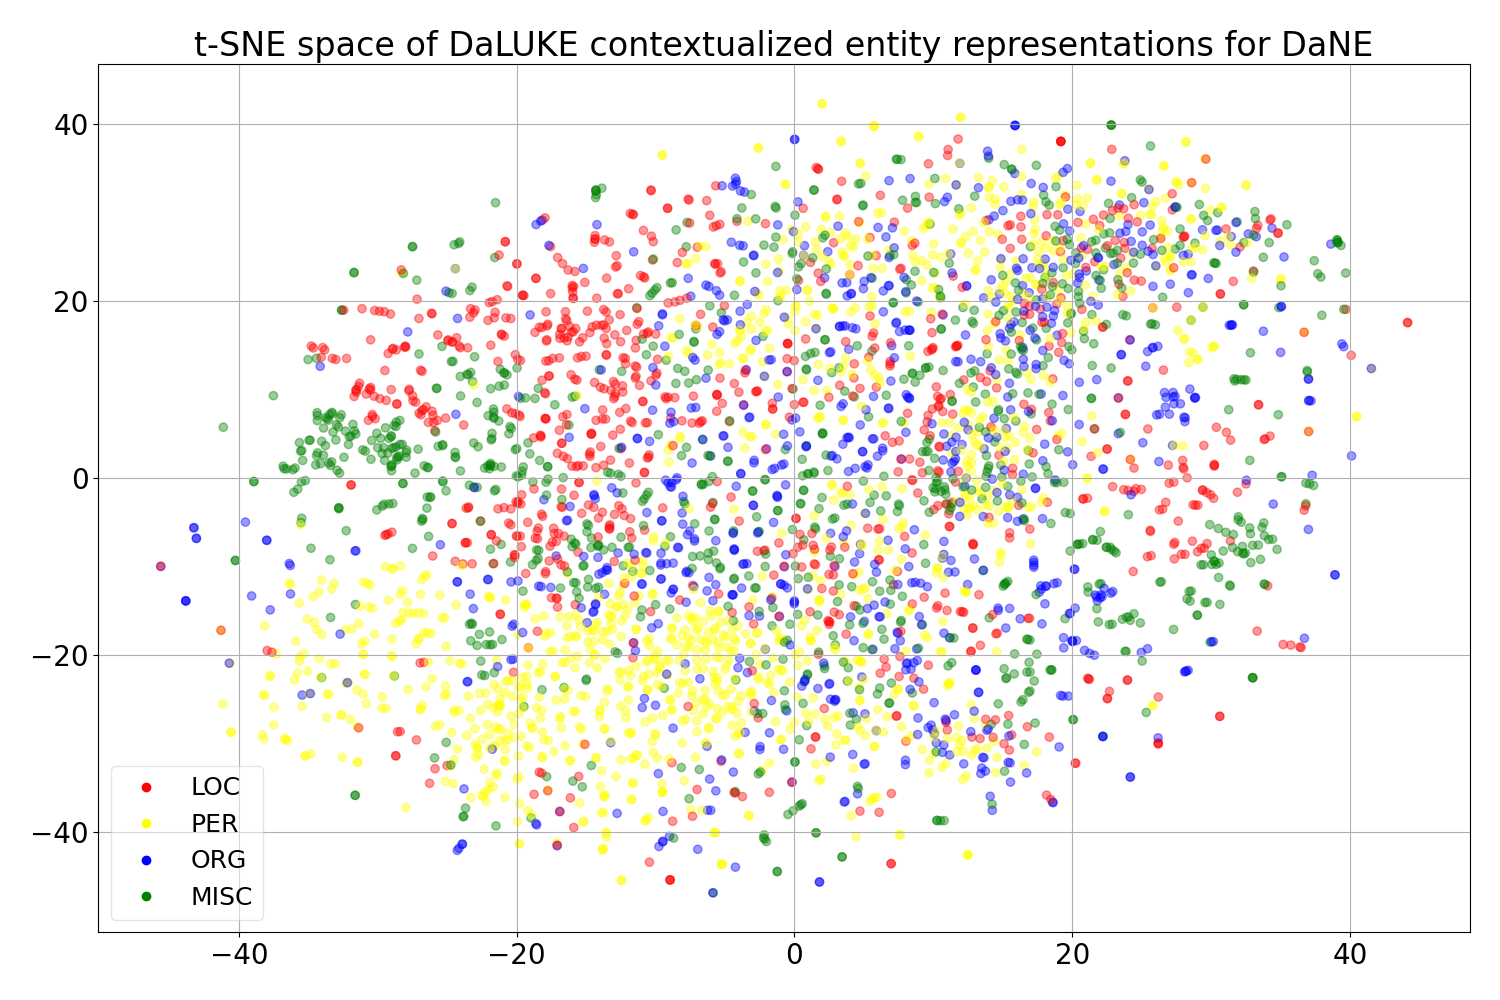
\includegraphics[width=0.7\linewidth]{full-geo/tsne}
    \caption{
        $t$-SNE performed on a 100K random subset of the full$\sim$ 1M possible entity spans in the training set of DaNE.
    }
    \label{fig:full-tsne}
\end{figure}\noindent

\begin{figure}[H]
    \centering
        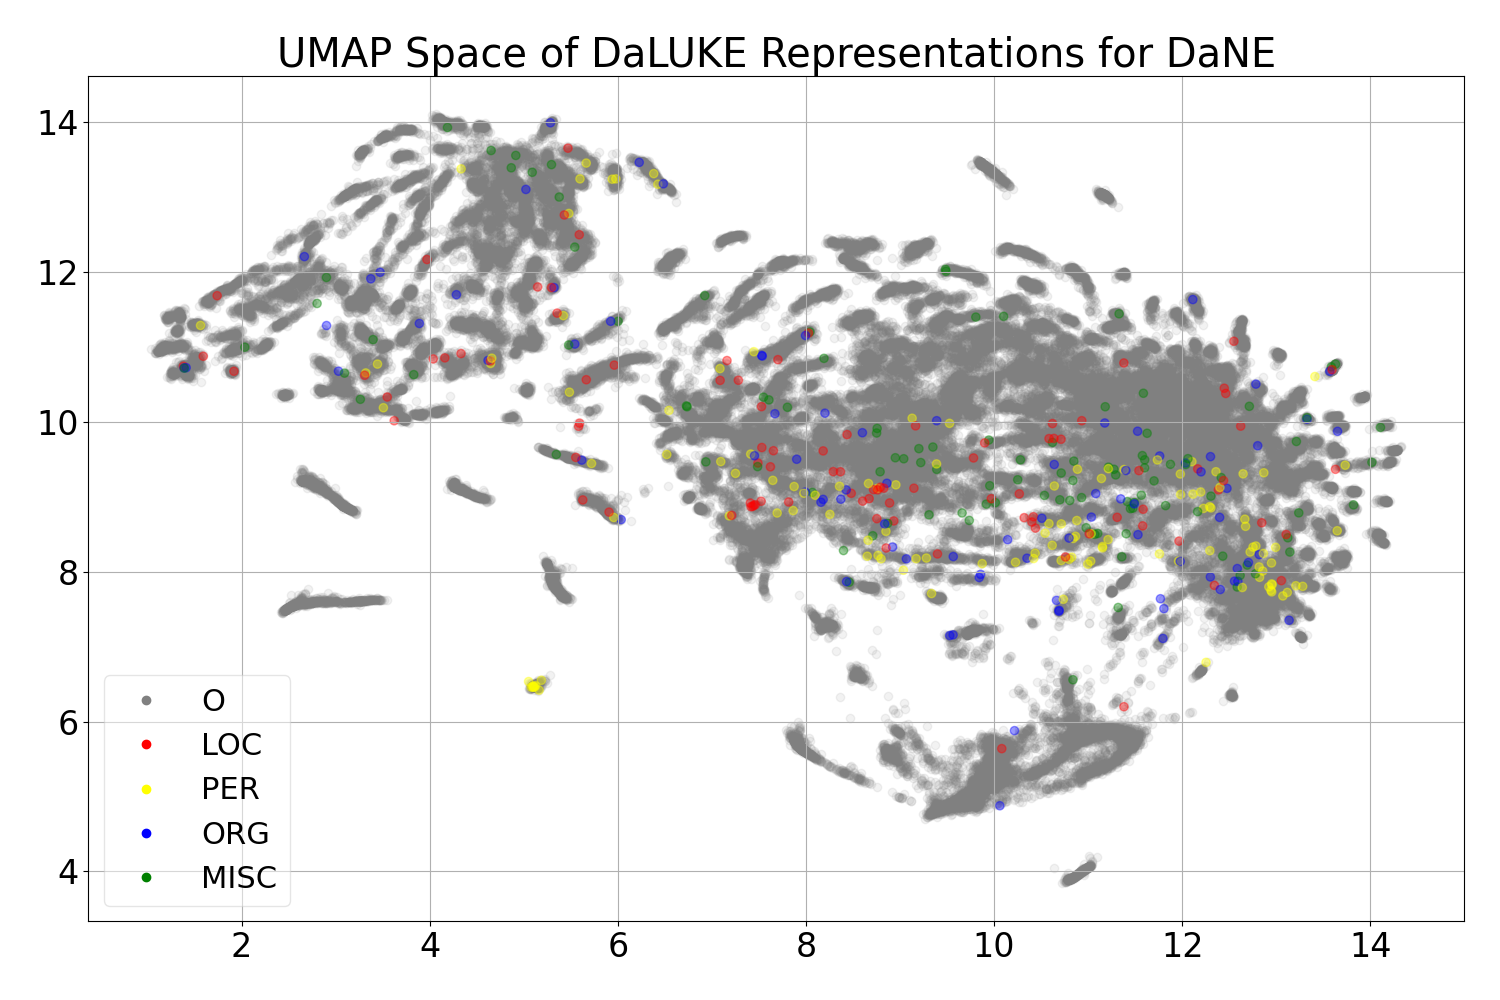
\includegraphics[width=0.7\linewidth]{full-geo/umap}
    \caption{
        UMAP performed on a 100K random subset of the full $\sim$ 1M possible entity spans in the DaNE training set.
    }
    \label{fig:full-umap}
\end{figure}\noindent

\begin{figure}[H]
    \centering
        \includegraphics[width=\linewidth]{full-geo/variance_explained}
    \caption{
        Variance explained by principal components found by PCA on full DaNE training dataset.
    }
    \label{fig:full-varex}
\end{figure}\noindent

\begin{figure}[H]
    \centering
        \includegraphics[width=\linewidth]{pos-geo/variance_explained}
    \caption{
        Variance explained by principal components found by PCA on the dataset including positive labels.
    }
    \label{fig:pos-varex}
\end{figure}\noindent

\end{document}
